\chapter{Implementaci\'on del sistema}
%
\section{Implementación Comunicación Humano Máquina}

Utilizando el software \textit{Nextion Editor} se diseñó una interfaz gráfica; la interfaz cuenta con 6 páginas: página principal, menú, configuración de hora actual, configuración de horarios de alimentación, ajuste de cantidad de gallinas y error.

La pantalla debe ser alimentada por una tensión de \SI{5}{\volt}, mientras que la tarjeta ESP32 es alimentada por una tensión de \SI{3.3}{\volt} y sus pines no pueden recibir más de  esa tensión. Por lo tanto, es necesario implementar un convertidor de nivel lógico bidireccional que está compuesto por un MOSFET y dos resistencias de \SI{10}{\kilo\ohm}.

Para la comunicación con la pantalla es requerido establecer un protocolo en la capa lógica que identifique mediante un código hexadecimal el inicio de transmisión de datos de la pantalla a la ESP32.

\subsubsection{Verificación}

Durante las pruebas, cada página funcionó adecuadamente, mostrando la información requerida. Los ajustes realizados en la pantalla se vieron reflejados en el monitor serial del IDE de Arduino; se hicieron pruebas dejando conectada la pantalla durante horas a fin de entender si entraba en un modo de reposo automático que pudiera interferir con las funciones, lo cual resultó correcto, se agregó un encendido automático de la pantalla de acuerdo a la rutina de alimentación; con las pruebas realizadas se determinó que la comunicación Humano Máquina es funcional.

\section{Almacenamiento de Alimento}

Se cortaron las tolvas de acuerdo a lo diseñado; sin embargo, se encontraron problemas al momento de doblar las piezas, encontrando que no era físicamente posible doblar la pieza sin que sufriera deformaciones; por lo que fue necesario hacer modificaciones al diseño de las piezas. 

Se separaron en cada una de sus caras, de tal manera que se unieran mediante remaches. 

Para la estructura se realizó según lo previsto uniendo los perfiles de acero mediante soldadura. Para reducir vibraciones se colocaron soportes de goma en las patas.

Las placas de acero se soldaron a la estructura dando estabilidad y soportando los elementos que contiene. se perforaron de acuerdo al diseño.



\subsubsection{Verificación}

El ensamble de las piezas del módulo no presentó fallos en soportar el peso y los componentes.


\section{Pesaje alimento}

El pesaje del alimento se realizó mediante una celda de carga de \SI{5}{kg}. Se utilizó un espárrago roscado de 1/2'' para empujar el alimento una vez termine de medir el peso; en conjunto con elementos fabricados mediante manufactura aditiva que sostienen el rodamiento y la tuerca del sistema.

\subsubsection{Verificación}

Se realizaron pruebas de pesaje con la báscula por separado, logrando medir con un error de \SI{0.5}{Kg}. El mecanismo de empuje presentó problemas al mover el alimento, por fricción con las paredes y la báscula. Se redujeron las dimensiones.

\section{Distribución de alimento}

Para los ejes que soportan la estructura fue necesario rectificarlos a $25 \text{ mm}$ debido a que únicamente se encontraron en medidas imperiales; utilizar rodamientos lineales (comúnmente llamados chumaceras) imperiales implicaría un costo mucho mayor; para su manufactura fue requerido el uso de la luneta móvil, elemento que permite mantener rectos elementos tan largos.

La transmisión de potencia entre el motor y el tornillo se propone la utilización de engranes para reducir el esfuerzo en el motor. Los cálculos para dichos engranes se pueden encontrar en el apéndice \ref{apendice3}.

Por cambios en los requerimientos, se realizó una estructura auxiliar que soporta las chumaceras, permitiendo el movimiento de la tolva a lo largo de los ejes que la soportan.

\subsubsection{Verificación}

El montaje de los elementos no presenta interferencias en el movimiento al lograr cumplir el recorrido de 1.5 m con los 3 kg de carga. En la imagen \ref{fig:MontajeDist} se muestra el montaje de la tolva en las flechas y el tornillo.

\begin{figure}[htbp]
    \centering
    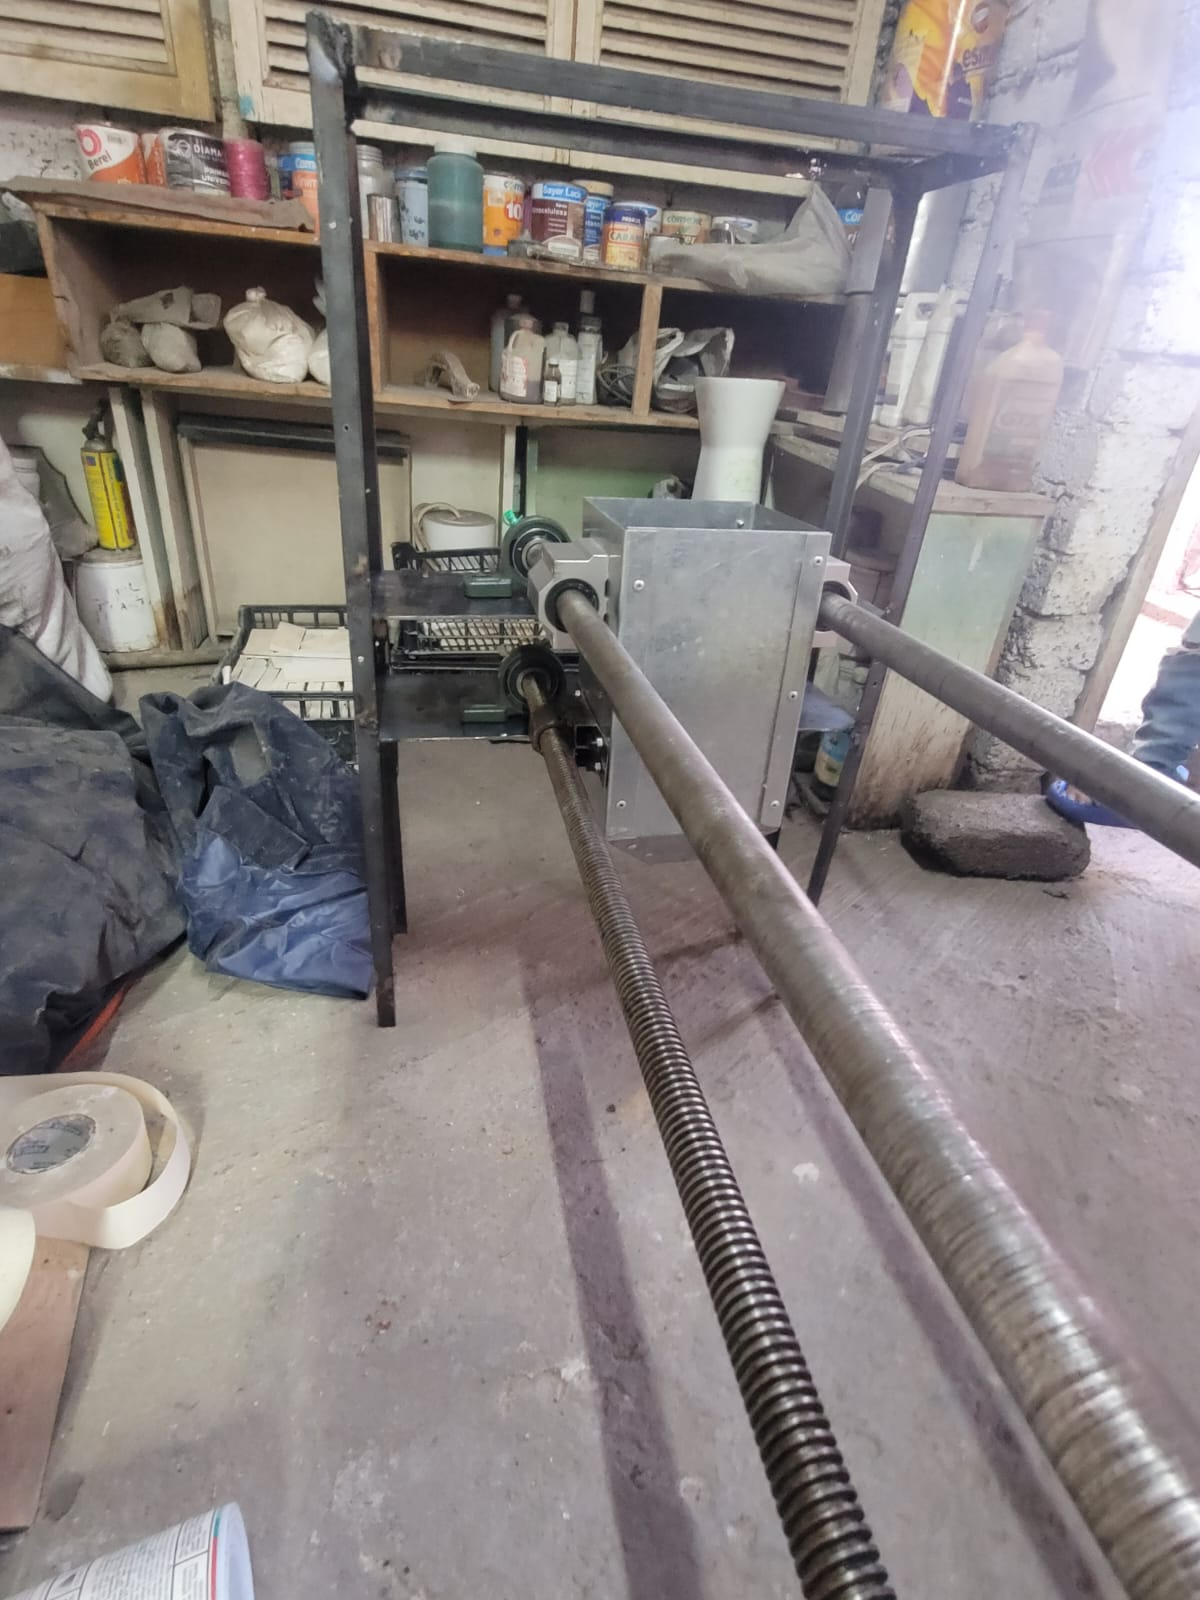
\includegraphics[width=0.75\linewidth]{imagenes/imacap/implementacion/SisFin1.jpeg}
    \caption{Montaje de elementos de distribución de alimento}
    \label{fig:MontajeDist}
\end{figure}

\section{Circuito sistema alimentación}

Para el circuito hubo que hacer muchas modificaciones al diseño original que se encontraba en la \ref{fig:ECA}, debido a que la ESP 32 es una tarjeta que debe alimentarse a \SI{3.3}{\volt}; mientras que la pantalla requiere de una alimentación de $5 \text{ V} $, en conjunto con su comunicación serial. Por lo que fue necesario el uso de un convertidor de nivel lógico, bidireccional, de $3.3 \text{ V}$ a $5 \text{ V}$ que se compone de un MOSFET y dos resistencias para cada línea de comunicación; se optó por esta solución debido a que se trata de comunicación serial y con el fin de a futuro poder utilizar frecuencias más altas.

Así mismo, se encontró que muchos de los pines de la tarjeta están reservados para funciones especiales, por lo que se redujo considerablemente la cantidad de periféricos. Considerando que para que el alimento pase del almacenamiento a la etapa de pesaje, se utiliza un motor de solenoide que abre y cierra una cuchilla, en conjunto con el motor de CD de la báscula y el motor NEMA, para cada motor es necesario el uso de $2$ sensores que marquen el inicio y el fin de carrera. Cada motor de CD requiere de $3$ señales, $2$ de dirección y una del PWM que controla la velocidad del motor. Se tendría en total el uso de $17$ pines de la tarjeta, lo que provocaría una alta demanda de corriente a la tarjeta. Por lo que la solución que se encontró fue el uso de demultiplexores y multiplexores para la lectura de los \textit{limit switch} y el control de cada motor.

Se optó por el uso de los integrados: , entre los que se encuentra  

El esquemático del circuito se puede ver en el apéndice 

\subsection{Verificación}

En una \textit{protoboard} se realizaron distintas pruebas del funcionamiento del circuito, integrando correctamente cada componente que se seleccionó. Se estableció el código para controlar el sistema basado en la imagen \ref{fig:DFSA} utilizando el entorno de Arduino IDE y programando en el lenguaje de C$++$. 

Cada etapa del programa fue probada individualmente mediante funciones que demostraban su correcto funcionamiento. Conectando los motores, la pantalla y los sensores a la tarjeta y verificando que cada elemento cumpliera su función. 

Posteriormente se realizó la integración del circuito en el sistema. 

Se miden corrientes de 2 A en el motor de solenoide que abre y cierra la tolva fija; y de hasta 4 A en el motor que mueve el alimento de la báscula a la tolva de distribución.


%\section{Registro de postura}

%Para el módulo de registro de postura se descartó el uso de la celda de carga debido a que se mostraron problemas al necesitar una recalibración constante. Debido a ello, para identificar la postura se hizo uso de un sistema de visión artificial que reconozca la firma del huevo, para reconocer si la gallina puso o no.

%También se encontraron problemas al implementar las etiquetas RFID debido a que funcionan a una frecuencia de \SI{134.2}{\kilo\hertz} la cual no cuenta con lectores de bajo costo; siendo las frecuencias más comerciales de \SI{125}{\kilo\hertz} y de \SI{13.2}{\mega\hertz}



%\subsection{Verificación}



%%%%%%fin del archivo
\endinput 